\documentclass[../report]{subfiles}
\setcounter{section}{0}
\begin{document}

本章では,本グループの取り組みの背景と目的を説明する.
\bunseki{佐藤碧}


\section{認知症の現状}
近年の我が国では,認知症患者数が増加傾向にある.
二宮(2014)によると,2012年時点で日本国内の推定認知症患者数は462万人であった\cite{syourai}.
2025年では675万人,2040年には802万人にまで上ると予想されている(図\ref{fig:ninchisyo-graph}).
また同研究によると,65歳以上の高齢者の推定認知症有病率は2012年では15.5%,2025年には20.6%,2040年には25.4%と,年々増加していくと予想されている\cite{syourai}.
\begin{figure}[htbp]
    \begin{center}
        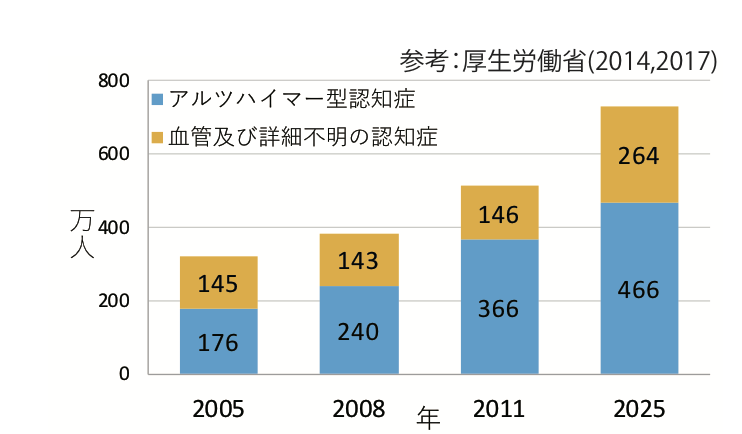
\includegraphics[width=10cm]{imgs/1_ninchisyo-graph.png}
        \caption{日本の認知症の総患者数の推移}
        \label{fig:ninchisyo-graph}
    \end{center}
\end{figure}
\bunseki{佐藤碧}


\section{認知症の発症原因} \label{sec:cause}
認知症は,その症状を引き起こす病気の種類によっていくつにも分類される.
例えば,「アルツハイマー病」「レビー小体型認知症」「前頭側頭型認知症」「脳血管性認知症」といったように分類される.
更に,それらの病気の原因として生活習慣病があげられる.
生活習慣病は従来より「脳血管性認知症」との関連が指摘されてきた.
だが近年の研究によって,生活習慣病は「アルツハイマー病」にも関連があり,その発症や進行に大きく関わっている事が明らかになってきた\cite{seikatsu}.
例えば,「高血圧」「糖尿病」「脂質異常病」といった生活習慣病が,認知症と関係があるとされている(図\ref{fig:relation-dementia-life-habit}).
\begin{figure}[htbp]
    \begin{center}
        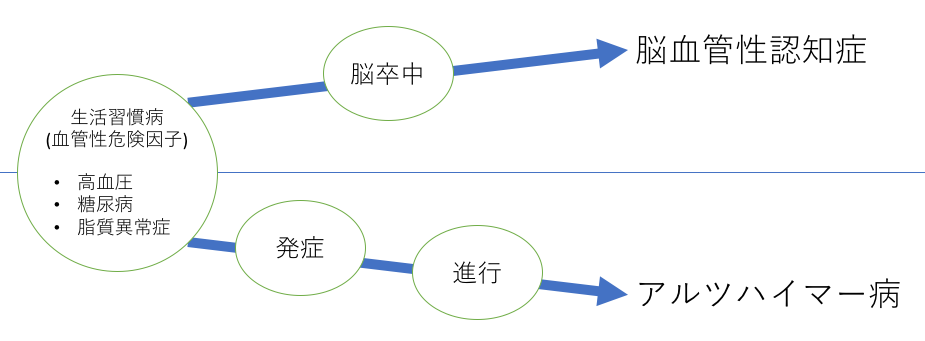
\includegraphics[width=10cm]{imgs/1_relation-dementia-life-habit.png}
        \caption{認知症と生活習慣病の関係}
        \label{fig:relation-dementia-life-habit}
    \end{center}
\end{figure}
\bunseki{佐藤碧}


\section{認知症と食習慣の関係}
\ref{sec:cause}でも述べたように,認知症は生活習慣病と関係がある.
「脳血管性認知症」は血管性の病気によって引き起こされる認知症である.
したがって,生活習慣病を予防して健康的な血管を維持できるようにすれば,「脳血管性認知症」の発症を抑えることが可能である.
また近年の縦断的疫学調査や5$\sim$10年にわたる大規模な追跡調査の結果では,「アルツハイマー症」には食事に含まれる栄養素が密接に関わっていると報告されている\cite{nutrition-dementia-00}\cite{nutrition-dementia-01}.
\bunseki{佐藤碧}


\section{認知症研究について}
認知症には,認知症患者が徘徊して自宅に戻れないという問題や,認知症患者数が年々増加傾向にあるということで介護者の負担が大きくなってきているという問題がある.
上記以外にも多くの問題が存在している認知症であるが,それらを解決するために行われている研究は,主に以下の4つに分類することができる.

\begin{enumerate}
    \item 認知症患者を対象とした,認知症の治療や患者の支援に関する研究
    \item 認知症患者をサポートする介護者を対象とした,介護の負担軽減に関する研究
    \item 認知症になる以前の人を対象とした,認知症予防に関する研究
    \item 認知症患者の家族や治療に当たる医師を対象にした,第三者による医療選択に関する研究
\end{enumerate}

例えば1.では,漢方を利用した認知症治療に関する研究\cite{dementia-prevention-with-chinese-medicine}や,リハビリによって在宅復帰に至る要因を明らかにしようとする研究\cite{rehabilitation}が挙げられる.
2.では,カメラシステムを用いた認知症高齢者の見守り支援を行う研究\cite{camera-system}が挙げられる.
3.では,複合型認知症予防プログラムの効果を明らかにしようとする研究\cite{dementia-prevention-with-some-programs}が挙げられる.
4.では,認知症治療における意思決定支援に関する研究\cite{medical-choice}が挙げられる.

上記のうち,特に3.の認知症予防に関する研究では,「認知症の予防には,日常生活の中でコミュニケーションを充実させて脳の機能を活性化することを心がけ,食事と運動のバランスをとる生活習慣病対策を意識したライフスタイルを実践することが大切である.」\cite{dementia-prevention},ということが明らかになっている.

そこで本グループは,認知症になる以前の人を対象として,高齢者でも簡単に扱えるようにユーザが行う操作を最小限にして食生活を管理できるシステムの開発を行った.
\bunseki{佐藤碧}


\section{目的} \label{sec:objective}
本グループは「認知症を予防すること」を大きな目的とし活動を進める.
そこで,1.3で挙げられた認知症と食習慣の関係に着目し,認知症になる前の段階の人(以下,対象者と記す)に向けて「食生活の改善をしてもらう」ことを目的に開発を行う.
そのため以下の内容により,食生活の見直しを促し,認知症予防を図ろうと考える.

\begin{itemize}
    \item 日々の食事を可視化し,蓄積された食事のデータを自身が閲覧する
    \item 他者から自身の食事に対するフィードバックを受ける
\end{itemize}

以上の内容を満たすため,本グループは「食生活を見直し認知症を予防するシステム,ふーろぐの開発」を行う.
具体的には,対象者に普段の食事を撮影し,写真というデータとして記録してもらう.
そのデータを自身閲覧,また対象者の家族や医療従事者に共有しメッセージを受け取ることができるシステムの開発を行う.
システムの流れは,まず高齢者でも簡単に撮影することができるように,本グループが作成するボックスに料理を置くだけで,自動的に写真の撮影ができる.
撮影した写真はテレビで閲覧することができる.
また,撮影した写真から栄養素を判断し,足りていない栄養を補えるような料理をテレビ画面から提案する.
一方で,対象者の家族や医療従事者は,Webから対象者が撮影した写真を閲覧することができる.
このとき,対象者が摂取した栄養素もチャート式で表示させる.
さらに,Web画面には対象者にメッセージを送信できる機能も加える.
メッセージが送信された場合には,対象者のテレビ画面にメッセージ内容が表示される.
これにより対象者は,自身の食生活に対するフィードバックを受け取ることができる.

これにより,対象者が食生活を簡単に記録でき,記録したデータを閲覧することができる.加えて,対象者は,他者からのフィードバックを受けることによって食生活の見直しができる.
また,医療従事者に記録したデータを提供することは,認知症になったときの意思決定支援に役立つと考える.
\bunseki{堀沙枝香}

\end{document}
